\chapter{Bijlage}



\noindent Verantwoording wegingen

\begin{figure}[h]
    \centering
    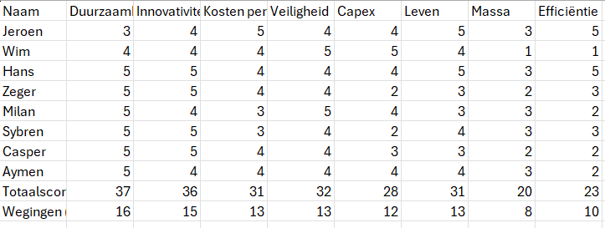
\includegraphics[width=0.5\linewidth]{tabel wegingen.png}
    \caption{Wegingen bepalen}
    \label{fig:wegingen}
\end{figure}

\subsection{Vergelijking van batterijen}
\begin{table}[h]
\centering
\caption{Vergelijking van batterijen \cite{Szewczyk2023}}
\begin{tabular}{lcccc}
\toprule
Batterijtype & Veiligheid & Kosten & Levensduur (cycli) & Energiedichtheid (Wh/kg) \\
\midrule
NMC & + & + & 1500 & 200 \\ 
LFP & ++ & + & 3000 & 120 \\ 
LTO & ++ & - - & 10000 & 80 \\
LCO & - - & + & 1000 & 200 \\
LMO & + & ++ & 700 & 150 \\
NCA & + & ++ & 500 & 260 \\
G-NMC & + & + & 8000 & 130 \\
\bottomrule
\end{tabular}
\label{tab:vergelijking_batterijen}
\end{table}


\begin{table}[h]
\centering
\caption{Vergelijking van energieopslagmethoden per eenheid}
\resizebox{\textwidth}{!}{
\begin{tabular}{lcccccc}
\toprule
Criterium & Weging (\%) & LFP & Zeezoutbatterij (gen 4.0) &  Waterstof (druk)  \\
\midrule
CAPEX (€) & 10 & 2.468,00 &   &\\
OPEX (€) & 10 & 1.4 & Is toch zelfde als LFP? Gewoon stroom, vgm geen onderhoud & \\
Massa (kg) & 5 & 40 & 18.7  & 1\\
Energiedichtheid/gewicht (Wh/kg) & -- &  145  & 25.89  & &\\
Energiedichtheid/volume (Wh/dm$^3$) & -- &180& 34.05  & \\
Efficiëntie (\%) & 10 & \approx 92 &97  & \\
Innovativiteit (\%) & 10 & 2.6 & 4.6 & 4.0 \\
Duurzaamheid (Score) & - & 3.94 & 5.00 & 3.72 & \\
Veiligheid  &  & 3.4 & 4.3 & 2.0 \\
\bottomrule
\end{tabular}
}
\label{tab:prestatievergelijking_uitgebreid}
\end{table}




\begin{table}[h]
\centering
\caption{Berekeningen van energieopslagmethoden per eenheid WORDT BIJLAGE}
\resizebox{\textwidth}{!}{
\begin{tabular}{lcccccc}
\toprule
Criterium & Weging (\%) & LFP & Zeezoutbatterij (gen 4.0) & Zeezoutbatterij (gen 6.0) & Waterstof (druk) \\
\midrule
CAPEX (€) & 10 & 2.468,00\cite{mg_price_list_2026}  &  & &\\
OPEX (€) & 10 & 0.24€/kWh \times 5.8 kWh \approx 1.4 \cite{mg_lfp_datasheets_page_2026}\cite{independer2026stroomprijs} & & &\\
Massa (kg) & 5 & 40 \cite{mg_lfp_datasheets_page_2026} &  Massa 1 cel is 146 g (0.4-2.0V), in elke batterij zitten 128 cellen, dus batterij (24 V, 20 Ah) weegt 18.7 kg & 1 & 1\\
Energiedichtheid/gewicht (Wh/kg) & -- & $\frac{5800Wh}{40kg}$ = 145 \cite{mg_lfp_datasheets_page_2026} & Gebaseerd op gravimetrische energiedichtheid (25.89 Wh/kg) & &\\
Energiedichtheid/volume (Wh/dm$^3$) & -- & $\frac{5800Wh}{2.95 dm \cdot 5.31 dm \cdot 2.06 dm}$ = 180 \cite{mg_lfp_datasheets_page_2026}& 34.05 & &\\
Efficiëntie (\%) & 10 & \approx 92 \cite{redondoiglesias2022efficiency}& 97& &\\
Innovativiteit (\%) & 10 & 2.6 & 4.6 &4.6 & 4.0 \\
Duurzaamheid (?) &  & &  & & \\
Veiligheid (1/5)  &  & 3.4 & 4.3 &  4.3 & 2.0 \\
\bottomrule

\end{tabular}
}
\label{tab:prestatievergelijking_uitgebreids}
\end{table}

\subsection{Opladen van zeezoutbatterij}

Tijdens het opladen is de volgende data gerealiseert:
\subsubsection{Setup}
For voltage measurement a multimeter is used.\\
For current measurement the gauge of the powersource is used.\\
Power source is an old (car)batterycharger. Can charge at 6V and 12V. We initialy set the power source to 6V.\\
surrounding temperature: 13degrees (outside temp, buienalarm, 17-5-26, 12:00, Baambrugge). battery is near an open window.\\
a test load (DC motor) is occacionaly used to determine if the load can be used for the actual test, and to read of the current with the multimeter, as it's probably more accurate than the gauge on the old charger.\\
During the experiment, at 11:54, two cables with small diameter are added to the circuits, to lower the charging current.

\subsubsection{\textbf{SSB charging log}}
start: 11:30
charge voltage:2.93v
charge current: 3.5A
\\\\
11:31: current keeps rising, now at 4 A\\
11:32: power shutoff, discharge current: 3.2A. discharge voltage 1.75\\
11:33: resume charging, 4A at 2.91V.\\
11:33: load checked, works.\\
11:35: heat check: no warmth discharge from the battery.\\
11:38: attempt to switch power source from 6V to 12V, current immediately rises to 6A (which is the max reading of the current gauge, so maybe more?). Actual voltage rises to 3.56.\\
11:38: switched back to 6V power source, so now charging at 2.87V, but current stays at 6+ A.\\
11:40: heat check of power soucre: slight warmth radiating from power source.\\
11:40: power source shut-off, attempt to let the load cycle. Battery doesn't yet have enough current. discharge power at steady 1.75V.\\
11:45: charging voltage has risen to 2.99V.\\
11:49: charging stopped. Power source is rated for 4A constant charging, where the battery continuously charged at 6+ A, for which the old power source wasn't designed.\\
11:49: heat check: no warmth discharge from battery. warmth discharge on power source slightly increased compared to previous measurement.\\
11:54: continue charging. Added some small cables inbetween to reduce charging current. Current is now at 2.4A, voltage at 4.04V.\\
11:55: power source makes small buzzing sound, probably also was there before, but didn't notice untill I checked.\\
11:55: tried to switch to 12V, current went to 4A, and voltage to 6.4V. However, as this is an old power source, charging at 4A continouusly will propbably damage it, so switched back to 6V.\\
11:57: charging at 4.17V, 2.2A.\\
11:58: voltage dropped to 3.85V, current still at 2.2A.\\
12:01: heat check: no warmth discharge from the battery, heat discharge from power source decreased. closed the window, it got cold and as the battery doesn't have any warmth discharge, no need for cooling.\\
12:01: voltage increased to 3.97V, current still 2.2A\\
12:03: voltage dropped to 3.89V, current 2.1A (current difference might be due to old equipment).\\
12:05: voltage increased to 3.91V, current 2.1A.\\
12:06: turned the multimeter upside down, then right side up, current now reads 4.01V.\\
12:12: steady charging at 4V, 2.1A. It also seems that the battery (4sacks in parallel, so 4 cells?) are rated for max 2.4A current, although the provided literature is a bit vague on what charging parameters to use. (is one sack one cell? And does "box of 4 blocks in parallel, 8 in series" mean box of 4 cells in parallel or 8 cells in series?\\
12:36: still charging at 4V, 2.1A.\\
12:36: heat check, seasalt battery has a very slight warmth, power source warmth decreased.\\
12:40: stopped charging, checked if battery can power load, which was succesfull.\\
12:42:'visual battery inspection. The leads of the cells seam to be rather soft, the clamps of the charger slightly deformed them.\\
12:45: amp test: output currently 0.27A.\\
12:52: resume normal charging. Due to slightly improves circuit, charging at 5.2V, 2.1A.\\
12:53: charged for approx 1hour, 0.27A.\\
13:03: charging at 5.3V,2.1A.\\
13:05 heat check: power source has negligible heat dissipation. Battery has slight heat dissipation, though only slightly sensible. Battery might have become a bit stiffer, although this has not been previously checked, and therefore can also not be the case. Small wires that where used start to heat up. might be wise to change them.\\
13:07: stop charging to swap out the small cables so they don't overheat.\\
13:08: discharge at 1.8V, which is quite good.\\
13:09: resumed charging, 5.4V at 2A. Swapped out the small cables for other ones of the same length, thickness, rating etc. old cables where cold already when I swapped them, and new ones where almost immediately the same temp as the old ones, so it seems to be just heat dissipation from the current, not accumulating heat, thus the cables do exactly what we want (act as additional resistance by dissipating heat). Connections of the multimeter have also improved, readings have become more stable.\\
13:41: steadily charging at 5.5V, 1.99A. slight local heat dissipation of the battery, though not even near concerning.\\
14:22: visual inspection: no notable differences.\\
14:22: heat inspection: heat dissipation from the battery increased more than previously measured. small cables are warm, but not concerning.\\
14:22: still charging at 5.5V, 2A. Even though the battery starts to warm up a bit, I would expect a drop in current when the battery is (almost) fully charged.\\
14:30: stopped charging.\\
14:30: voltage test: open circuit is 1.7V, closed circuit with load is 1.1V. Should the closed circuit lpad be 1.7V as well when fully charged?\\
14:33: resumed charging, 5.5V, 2A.\\
14:40: visual inspection: I noticed some hardened droplets on the top of the cells. They could just be adhesive used to seal the bags, but they might also be leakeage? Luckily, as this is a seasalt battery, there shouldn't be any harm to me.\\
14:45: stopped charging, ending the charging. The battery should be sufficiently charged for the upcomming test. \\
19:19: upon visual inspection: under certain light angle, slight yellow discoloration can be seen, although very slight. 


\subsubsection{\textbf{Looking back}}
The initial current of 6+ A at 3V is in line with the fact that the battery was deeply discharged. Also in line is the fact that, when the battery gains charge, the voltage increases and the current drops. According to the manufacturer, the charging time would be approximately eight hours. However, with three hours of charging, the battery should have enough charge for the experiment. Visualy inspecting the battery later, showed yellow coloring in the battery. According to the manufacturer this is due to crystals forming due to slight (local?) overcharging. however, In literature it is stated that a drop in charging current and rise in voltage should occur when the battery is near-full, which hasn't happened. This would lead to the conclusion that the battery might not have been optimaly functioning. However, this likely won't affect the experiment, as long as it keeps enough charge to complete the experiment.

\subsubsection{\textbf{For the future}}
The material of the poles are very soft, electrical clamps damage the surface and deform it. Furthermore, the poles aren't guarded, so putting them in a bag for traveling could create a current through the bag if the material is conducting. Therefore, for future experiments with similar cells I would advise to create a simple, hard plastic case and additional poles of a stronger metal.


\subsection{Volledige metingen experiment}
\begin{table}[htbp]
\centering
\caption{Volledige meetreeks voor de Hard Rocking conditie}
\label{tab:hard_rocking_data}
\begin{tabular}{c S[table-format=2.2] S[table-format=1.2] S[table-format=2.3]}
\toprule
\textbf{Meting (\#)} & {\textbf{Stroom I (mA)}} & {\textbf{Spanning V (V)}} & {\textbf{Vermogen P (mW)}} \\
\midrule
1  & 19.49 & 1.72 & 33.523 \\
2  & 19.93 & 1.72 & 34.280 \\
3  & 19.54 & 1.72 & 33.609 \\
4  & 19.61 & 1.72 & 33.729 \\
5  & 19.52 & 1.72 & 33.574 \\
6  & 19.56 & 1.73 & 33.839 \\
7  & 19.55 & 1.72 & 33.626 \\
8  & 19.58 & 1.72 & 33.678 \\
9  & 19.50 & 1.72 & 33.540 \\
10 & 19.46 & 1.72 & 33.471 \\
11 & 19.53 & 1.72 & 33.592 \\
12 & 19.51 & 1.72 & 33.557 \\
13 & 19.52 & 1.73 & 33.770 \\
14 & 19.58 & 1.73 & 33.873 \\
15 & 19.54 & 1.72 & 33.609 \\
16 & 19.57 & 1.72 & 33.660 \\
17 & 19.53 & 1.72 & 33.592 \\
18 & 19.51 & 1.72 & 33.557 \\
19 & 19.54 & 1.72 & 33.609 \\
20 & 19.50 & 1.72 & 33.540 \\
21 & 19.54 & 1.72 & 33.609 \\
22 & 19.62 & 1.72 & 33.746 \\
23 & 19.49 & 1.72 & 33.523 \\
24 & 19.46 & 1.73 & 33.666 \\
25 & 19.98 & 1.72 & 34.366 \\
26 & 19.48 & 1.72 & 33.506 \\
27 & 19.58 & 1.72 & 33.678 \\
28 & 19.52 & 1.72 & 33.574 \\
29 & 19.95 & 1.72 & 34.314 \\
30 & 19.53 & 1.72 & 33.592 \\
31 & 19.47 & 1.73 & 33.683 \\
32 & 19.42 & 1.73 & 33.597 \\
33 & 19.47 & 1.72 & 33.488 \\
34 & 19.56 & 1.72 & 33.643 \\
35 & 19.55 & 1.72 & 33.626 \\
36 & 19.56 & 1.72 & 33.643 \\
37 & 19.68 & 1.72 & 33.850 \\
38 & 19.54 & 1.72 & 33.609 \\
39 & 19.51 & 1.72 & 33.557 \\
40 & 19.65 & 1.72 & 33.798 \\
41 & 19.51 & 1.72 & 33.557 \\
42 & 19.47 & 1.72 & 33.488 \\
43 & 19.55 & 1.72 & 33.626 \\
44 & 19.48 & 1.72 & 33.506 \\
45 & 19.49 & 1.72 & 33.523 \\
46 & 19.56 & 1.72 & 33.643 \\
47 & 19.54 & 1.72 & 33.609 \\
48 & 19.48 & 1.72 & 33.506 \\
49 & 19.45 & 1.72 & 33.454 \\
50 & 19.48 & 1.73 & 33.700 \\
51 & 19.48 & 1.73 & 33.700 \\
52 & 19.58 & 1.73 & 33.873 \\
53 & 19.59 & 1.72 & 33.695 \\
54 & 19.96 & 1.72 & 34.331 \\
55 & 19.51 & 1.72 & 33.557 \\
56 & 19.52 & 1.72 & 33.574 \\
57 & 19.58 & 1.72 & 33.678 \\
58 & 19.49 & 1.72 & 33.523 \\
59 & 19.49 & 1.72 & 33.523 \\
60 & 19.48 & 1.72 & 33.506 \\
\bottomrule
\end{tabular}
\end{table}
\begin{table}[htbp]
\centering
\caption{Volledige meetreeks voor de Light Rocking conditie}
\label{tab:light_rocking_data}
\begin{tabular}{c S[table-format=2.2] S[table-format=1.2] S[table-format=2.3]}
\toprule
\textbf{Meting (\#)} & {\textbf{Stroom I (mA)}} & {\textbf{Spanning V (V)}} & {\textbf{Vermogen P (mW)}} \\
\midrule
1  & 19.60 & 1.72 & 33.712 \\
2  & 19.60 & 1.72 & 33.712 \\
3  & 19.60 & 1.72 & 33.712 \\
4  & 19.60 & 1.73 & 33.908 \\
5  & 19.60 & 1.72 & 33.712 \\
6  & 19.60 & 1.72 & 33.712 \\
7  & 19.60 & 1.73 & 33.908 \\
8  & 19.60 & 1.72 & 33.712 \\
9  & 19.50 & 1.73 & 33.735 \\
10 & 19.60 & 1.72 & 33.712 \\
11 & 19.50 & 1.72 & 33.540 \\
12 & 19.60 & 1.72 & 33.712 \\
13 & 19.60 & 1.72 & 33.712 \\
14 & 19.60 & 1.72 & 33.712 \\
15 & 19.60 & 1.72 & 33.712 \\
16 & 19.60 & 1.72 & 33.712 \\
17 & 19.50 & 1.72 & 33.540 \\
18 & 19.60 & 1.73 & 33.908 \\
19 & 19.50 & 1.72 & 33.540 \\
20 & 19.60 & 1.72 & 33.712 \\
21 & 19.50 & 1.72 & 33.540 \\
22 & 19.60 & 1.72 & 33.712 \\
23 & 19.60 & 1.72 & 33.712 \\
24 & 19.60 & 1.72 & 33.712 \\
25 & 19.60 & 1.72 & 33.712 \\
26 & 19.60 & 1.73 & 33.908 \\
27 & 19.50 & 1.72 & 33.540 \\
28 & 19.60 & 1.72 & 33.712 \\
29 & 19.60 & 1.72 & 33.712 \\
30 & 19.60 & 1.73 & 33.908 \\
31 & 19.50 & 1.72 & 33.540 \\
32 & 19.60 & 1.72 & 33.712 \\
33 & 19.60 & 1.72 & 33.712 \\
34 & 19.60 & 1.73 & 33.908 \\
35 & 19.60 & 1.72 & 33.712 \\
36 & 19.50 & 1.72 & 33.540 \\
37 & 19.60 & 1.72 & 33.712 \\
38 & 19.60 & 1.72 & 33.712 \\
39 & 19.60 & 1.73 & 33.908 \\
40 & 19.50 & 1.72 & 33.540 \\
41 & 19.60 & 1.72 & 33.712 \\
42 & 19.60 & 1.72 & 33.712 \\
43 & 19.50 & 1.73 & 33.735 \\
44 & 19.60 & 1.72 & 33.712 \\
45 & 19.50 & 1.72 & 33.540 \\
46 & 19.60 & 1.72 & 33.712 \\
47 & 19.60 & 1.72 & 33.712 \\
48 & 19.50 & 1.72 & 33.540 \\
49 & 19.60 & 1.72 & 33.712 \\
50 & 19.60 & 1.72 & 33.712 \\
51 & 19.50 & 1.72 & 33.540 \\
52 & 19.60 & 1.73 & 33.908 \\
53 & 19.50 & 1.72 & 33.540 \\
54 & 19.60 & 1.72 & 33.712 \\
55 & 19.50 & 1.72 & 33.540 \\
56 & 19.60 & 1.72 & 33.712 \\
57 & 19.50 & 1.72 & 33.540 \\
58 & 19.60 & 1.72 & 33.712 \\
59 & 19.50 & 1.72 & 33.540 \\
60 & 19.50 & 1.72 & 33.540 \\
\bottomrule
\end{tabular}
\end{table}
\begin{table}[htbp]
\centering
\caption{Volledige meetreeks voor de Static 0$^\circ$ (null) conditie}
\label{tab:static_0deg_data}
\begin{tabular}{c S[table-format=2.2] S[table-format=1.2] S[table-format=2.3]}
\toprule
\textbf{Meting (\#)} & {\textbf{Stroom I (mA)}} & {\textbf{Spanning V (V)}} & {\textbf{Vermogen P (mW)}} \\
\midrule
1  & 19.30 & 1.72 & 33.196 \\
2  & 19.23 & 1.72 & 33.076 \\
3  & 19.33 & 1.72 & 33.248 \\
4  & 19.50 & 1.72 & 33.540 \\
5  & 19.39 & 1.73 & 33.545 \\
6  & 19.42 & 1.72 & 33.402 \\
7  & 19.40 & 1.72 & 33.368 \\
8  & 19.45 & 1.72 & 33.454 \\
9  & 19.40 & 1.72 & 33.368 \\
10 & 19.36 & 1.72 & 33.299 \\
11 & 19.40 & 1.72 & 33.368 \\
12 & 19.48 & 1.72 & 33.506 \\
13 & 19.99 & 1.72 & 34.383 \\
14 & 19.26 & 1.72 & 33.127 \\
15 & 19.30 & 1.73 & 33.389 \\
16 & 19.38 & 1.72 & 33.334 \\
17 & 19.36 & 1.72 & 33.299 \\
18 & 19.46 & 1.72 & 33.471 \\
19 & 19.44 & 1.72 & 33.437 \\
20 & 19.35 & 1.72 & 33.282 \\
21 & 19.29 & 1.72 & 33.179 \\
22 & 19.38 & 1.72 & 33.334 \\
23 & 19.30 & 1.72 & 33.196 \\
24 & 19.31 & 1.72 & 33.213 \\
25 & 19.44 & 1.72 & 33.437 \\
26 & 19.29 & 1.72 & 33.179 \\
27 & 19.33 & 1.72 & 33.248 \\
28 & 19.40 & 1.72 & 33.368 \\
29 & 19.37 & 1.73 & 33.510 \\
30 & 19.34 & 1.72 & 33.265 \\
31 & 19.35 & 1.72 & 33.282 \\
32 & 19.37 & 1.72 & 33.316 \\
33 & 19.40 & 1.73 & 33.562 \\
34 & 19.34 & 1.72 & 33.265 \\
35 & 19.44 & 1.72 & 33.437 \\
36 & 19.41 & 1.72 & 33.385 \\
37 & 19.35 & 1.72 & 33.282 \\
38 & 19.38 & 1.72 & 33.334 \\
39 & 19.39 & 1.72 & 33.351 \\
40 & 19.32 & 1.72 & 33.230 \\
41 & 19.34 & 1.72 & 33.265 \\
42 & 19.40 & 1.72 & 33.368 \\
43 & 19.43 & 1.72 & 33.420 \\
44 & 19.36 & 1.72 & 33.299 \\
45 & 19.34 & 1.72 & 33.265 \\
46 & 19.34 & 1.72 & 33.265 \\
47 & 19.32 & 1.72 & 33.230 \\
48 & 19.34 & 1.72 & 33.265 \\
49 & 19.32 & 1.72 & 33.230 \\
50 & 19.34 & 1.73 & 33.458 \\
51 & 19.40 & 1.72 & 33.368 \\
52 & 19.29 & 1.72 & 33.179 \\
53 & 19.38 & 1.72 & 33.334 \\
54 & 19.28 & 1.72 & 33.162 \\
55 & 19.41 & 1.72 & 33.385 \\
56 & 19.30 & 1.72 & 33.196 \\
57 & 19.30 & 1.72 & 33.196 \\
58 & 19.30 & 1.72 & 33.196 \\
59 & 19.30 & 1.72 & 33.196 \\
60 & 19.30 & 1.73 & 33.389 \\
\bottomrule
\end{tabular}
\end{table}
\begin{table}[htbp]
\centering
\caption{Volledige meetreeks voor de Static 45$^\circ$ conditie}
\label{tab:static_45deg_data}
\begin{tabular}{c S[table-format=2.2] S[table-format=1.2] S[table-format=2.3]}
\toprule
\textbf{Meting (\#)} & {\textbf{Stroom I (mA)}} & {\textbf{Spanning V (V)}} & {\textbf{Vermogen P (mW)}} \\
\midrule
1  & 19.43 & 1.72 & 33.420 \\
2  & 19.35 & 1.73 & 33.475 \\
3  & 19.41 & 1.72 & 33.385 \\
4  & 19.48 & 1.72 & 33.506 \\
5  & 19.34 & 1.72 & 33.265 \\
6  & 19.18 & 1.72 & 32.990 \\
7  & 19.37 & 1.72 & 33.316 \\
8  & 19.38 & 1.72 & 33.334 \\
9  & 19.35 & 1.72 & 33.282 \\
10 & 19.44 & 1.72 & 33.437 \\
11 & 19.46 & 1.73 & 33.666 \\
12 & 19.39 & 1.72 & 33.351 \\
13 & 19.42 & 1.73 & 33.597 \\
14 & 19.39 & 1.73 & 33.545 \\
15 & 19.43 & 1.72 & 33.420 \\
16 & 19.98 & 1.73 & 34.565 \\
17 & 19.43 & 1.72 & 33.420 \\
18 & 19.98 & 1.72 & 34.366 \\
19 & 19.91 & 1.72 & 34.245 \\
20 & 19.37 & 1.72 & 33.316 \\
21 & 19.24 & 1.72 & 33.093 \\
22 & 19.91 & 1.72 & 34.245 \\
23 & 19.40 & 1.72 & 33.368 \\
24 & 19.44 & 1.73 & 33.631 \\
25 & 19.45 & 1.72 & 33.454 \\
26 & 19.33 & 1.73 & 33.441 \\
27 & 19.28 & 1.72 & 33.162 \\
28 & 19.37 & 1.72 & 33.316 \\
29 & 19.40 & 1.72 & 33.368 \\
30 & 19.35 & 1.72 & 33.282 \\
31 & 19.35 & 1.72 & 33.282 \\
32 & 19.38 & 1.72 & 33.334 \\
33 & 19.31 & 1.73 & 33.406 \\
34 & 19.40 & 1.72 & 33.368 \\
35 & 19.37 & 1.72 & 33.316 \\
36 & 19.19 & 1.73 & 33.199 \\
37 & 19.35 & 1.72 & 33.282 \\
38 & 19.31 & 1.72 & 33.213 \\
39 & 19.22 & 1.72 & 33.058 \\
40 & 19.32 & 1.72 & 33.230 \\
41 & 19.32 & 1.72 & 33.230 \\
42 & 19.31 & 1.72 & 33.213 \\
43 & 19.39 & 1.72 & 33.351 \\
44 & 19.39 & 1.72 & 33.351 \\
45 & 19.98 & 1.72 & 34.366 \\
46 & 19.48 & 1.72 & 33.506 \\
47 & 19.92 & 1.72 & 34.262 \\
48 & 19.37 & 1.72 & 33.316 \\
49 & 19.40 & 1.72 & 33.368 \\
50 & 19.37 & 1.72 & 33.316 \\
51 & 19.34 & 1.72 & 33.265 \\
52 & 19.47 & 1.72 & 33.488 \\
53 & 19.23 & 1.73 & 33.268 \\
54 & 19.29 & 1.72 & 33.179 \\
55 & 19.22 & 1.73 & 33.251 \\
56 & 19.32 & 1.72 & 33.230 \\
57 & 19.35 & 1.73 & 33.475 \\
58 & 19.31 & 1.72 & 33.213 \\
59 & 19.46 & 1.72 & 33.471 \\
60 & {---}  & {---} & {---}   \\
\bottomrule
\end{tabular}
\end{table}
\begin{table}[htbp]
\centering
\caption{Volledige meetreeks voor de Static 90$^\circ$ conditie}
\label{tab:static_90deg_data}
\begin{tabular}{c S[table-format=2.2] S[table-format=1.2] S[table-format=2.3]}
\toprule
\textbf{Meting (\#)} & {\textbf{Stroom I (mA)}} & {\textbf{Spanning V (V)}} & {\textbf{Vermogen P (mW)}} \\
\midrule
1  & 19.55 & 1.72 & 33.626 \\
2  & 19.26 & 1.72 & 33.127 \\
3  & 19.34 & 1.72 & 33.265 \\
4  & 19.37 & 1.72 & 33.316 \\
5  & 19.38 & 1.72 & 33.334 \\
6  & 19.34 & 1.72 & 33.265 \\
7  & 19.28 & 1.72 & 33.162 \\
8  & 19.29 & 1.72 & 33.179 \\
9  & 19.34 & 1.72 & 33.265 \\
10 & 19.30 & 1.72 & 33.196 \\
11 & 19.31 & 1.72 & 33.213 \\
12 & 19.29 & 1.73 & 33.372 \\
13 & 19.34 & 1.72 & 33.265 \\
14 & 19.33 & 1.72 & 33.248 \\
15 & 19.40 & 1.72 & 33.368 \\
16 & 19.36 & 1.72 & 33.299 \\
17 & 19.32 & 1.72 & 33.230 \\
18 & 19.34 & 1.72 & 33.265 \\
19 & 19.34 & 1.72 & 33.265 \\
20 & 19.27 & 1.72 & 33.144 \\
21 & 19.34 & 1.72 & 33.265 \\
22 & 19.31 & 1.72 & 33.213 \\
23 & 19.38 & 1.72 & 33.334 \\
24 & 19.36 & 1.72 & 33.299 \\
25 & 19.40 & 1.72 & 33.368 \\
26 & 19.34 & 1.72 & 33.265 \\
27 & 19.34 & 1.72 & 33.265 \\
28 & 19.31 & 1.72 & 33.213 \\
29 & 19.36 & 1.73 & 33.493 \\
30 & 19.34 & 1.72 & 33.265 \\
31 & 19.35 & 1.72 & 33.282 \\
32 & 19.37 & 1.72 & 33.316 \\
33 & 19.40 & 1.73 & 33.562 \\
34 & 19.34 & 1.72 & 33.265 \\
35 & 19.44 & 1.72 & 33.437 \\
36 & 19.41 & 1.72 & 33.385 \\
37 & 19.35 & 1.72 & 33.282 \\
38 & 19.38 & 1.72 & 33.334 \\
39 & 19.39 & 1.72 & 33.351 \\
40 & 19.32 & 1.72 & 33.230 \\
41 & 19.34 & 1.72 & 33.265 \\
42 & 19.40 & 1.72 & 33.368 \\
43 & 19.43 & 1.72 & 33.420 \\
44 & 19.36 & 1.72 & 33.299 \\
45 & 19.34 & 1.72 & 33.265 \\
46 & 19.34 & 1.72 & 33.265 \\
47 & 19.32 & 1.72 & 33.230 \\
48 & 19.34 & 1.72 & 33.265 \\
49 & 19.32 & 1.72 & 33.230 \\
50 & 19.34 & 1.73 & 33.458 \\
51 & 19.40 & 1.72 & 33.368 \\
52 & 19.29 & 1.72 & 33.179 \\
53 & 19.38 & 1.72 & 33.334 \\
54 & 19.28 & 1.72 & 33.162 \\
55 & 19.41 & 1.72 & 33.385 \\
56 & 19.30 & 1.72 & 33.196 \\
57 & 19.30 & 1.72 & 33.196 \\
58 & 19.30 & 1.72 & 33.196 \\
59 & 19.30 & 1.72 & 33.196 \\
60 & 19.30 & 1.73 & 33.389 \\
\bottomrule
\end{tabular}
\end{table}

\section{Berekeningen energieopslagmethoden}
Rekening houden met het feit dat de hoeveelheid dat de ontladingsdiepte van een LFP batterij 80\% is om ervoor te zorgen dat de efficiëntie niet overmatig afneemt. Rekening houdend met de totale benodigde capaciteit van 108.15 kWh is er dan: 
\begin{equation}
E_{\text{bruto, LFP}} = \frac{E_{\text{totaal, inclusief reserve}}}{\text{DoD}} = \frac{108{,}15 \text{ kWh}}{0{,}80} = 135{,}1875 \text{ kWh}
\end{equation}

Vanuit Tabel 5.7 is te zien dat een enkele LFP-batterijmodule een nominale capaciteit heeft van $5{,}8 \text{ kWh}$ met een energetische efficiëntie van $92\%$ ($\eta = 0{,}92$).  Om de interne energieverliezen van de batterij te compenseren, moet de bruto benodigde capaciteit worden gecorrigeerd met de efficiëntie. Hierdoor stijgt de minimaal te installeren accucapaciteit ($E_{\text{geïnstalleerd}}$):

\begin{equation}
E_{\text{geïnstalleerd}} = \frac{E_{\text{bruto, LFP}}}{\eta} = \frac{135{,}1875 \text{ kWh}}{0{,}92} \approx 146{,}9429 \text{ kWh}
\end{equation}

\subsubsection*{Berekening van het aantal benodigde modules}
Het exacte aantal benodigde LFP-modules ($N_{\text{modules}}$) wordt bepaald door de totale geïnstalleerde capaciteit te delen door de capaciteit van één module ($E_{\text{module}} = 5{,}8 \text{ kWh}$):
\begin{equation}
N_{\text{modules}} = \frac{E_{\text{geïnstalleerd}}}{E_{\text{module}}} = \frac{146{,}9429 \text{ kWh}}{5{,}8 \text{ kWh}} \approx 25{,}335
\end{equation}

\noindent Aangezien er alleen hele modules geplaatst kunnen worden, wordt dit getal naar boven afgerond op een minimum van \textbf{26 modules}. Dit resulteert in een werkelijk geïnstalleerd vermogen van $26 \times 5{,}8 \text{ kWh} = 150{,}8 \text{ kWh}$.

\subsubsection*{Totale massa van het accupakket}
Met een individuele massa van $40 \text{ kg}$ per module uit Tabel 5.7, wordt de totale massa van het accupakket ($M_{\text{totaal}}$):
\begin{equation}
M_{\text{totaal}} = N_{\text{modules, afgerond}} \times 40 \text{ kg} = 26 \times 40 \text{ kg} = 1040 \text{ kg} \quad (1{,}04 \text{ ton})
\end{equation}

\subsubsection*{Totaal volume van het accupakket}
Volgens Tabel 5.7 zijn de dimensies van één module $0{,}531 \text{ m} \times 0{,}0206 \text{ m} \times 0{,}295 \text{ m}$. Het volume van één enkele module ($V_{\text{module}}$) bedraagt:
\begin{equation}
V_{\text{module}} = 0{,}531 \text{ m} \times 0{,}206 \text{ m} \times 0{,}295 \text{ m} \approx 0{,}03227 \text{ m}^3
\end{equation}

\noindent Het totale fysieke volume dat de 26 modules samen innemen ($V_{\text{totaal}}$) is dan:
\begin{equation}
V_{\text{totaal}} = N_{\text{modules, afgerond}} \times V_{\text{module}} = 26 \times 0{,}03227 \text{ m}^3 \approx 0{,}8390 \text{ m}^3
\end{equation}

\noindent Om de levensduur van de batterijsystemen te vergelijken met de brandstofcel, wordt het maximaal aantal laadcycli omgerekend naar de totale levensduur in jaren ($L_{\text{jaren}}$). Hierbij wordt uitgegaan van het operationele profiel van 40 vaardagen per jaar, waarbij elke vaardag gelijkstaat aan exact 1 volledige laadcyclus ($N_{\text{cycli/jaar}} = 40$).
De theoretische levensduur van het LFP-accupakket ($L_{\text{jaren, LFP}}$) op basis van de maximale degradatiegrens van $3500 \text{ cycli}$ bedraagt:
\begin{equation}
L_{\text{jaren, LFP}} = \frac{\text{Totale cycli LFP}}{N_{\text{cycli/jaar}}} = \frac{3500 \text{ cycli}}{40 \text{ cycli/jaar}} = 87{,}5 \text{ jaar}
\end{equation}

\noindent Vanuit Tabel 5.7 is te zien dat een enkele zeezoutbatterijmodule (gen 4.0) een nominale capaciteit heeft van $0{,}48 \text{ kWh}$ met een energetische efficiëntie van $97\%$ ($\eta = 0{,}97$). Omdat zeezoutbatterijen volledig ontladen mogen worden zonder degradatie van de chemie, is de ontladingsdiepte vastgesteld op $100\%$ ($\text{DoD} = 1{,}00$).

\subsubsection*{Correctie voor ontladingsdiepte (DoD)}
Aangezien de batterij volledig ontladen mag worden, is er voor de ontladingsdiepte geen extra overdimensionering van de bruto accucapaciteit ($E_{\text{bruto, zeezout}}$) vereist ten opzichte van de netto energievraag inclusief reserve ($108{,}15 \text{ kWh}$):
\begin{equation}
E_{\text{bruto, zeezout}} = \frac{E_{\text{totaal, inclusief reserve}}}{\text{DoD}} = \frac{108{,}15 \text{ kWh}}{1{,}00} = 108{,}15 \text{ kWh}
\end{equation}

\subsubsection*{Correctie voor batterij-efficiëntie}
Om de interne thermische en chemische energieverliezen tijdens het ontladen op te vangen, moet de bruto capaciteit worden gecorrigeerd met de energetische efficiëntie van $97\%$. Hierdoor stijgt de minimaal te installeren accucapaciteit ($E_{\text{geïnstalleerd}}$):
\begin{equation}
E_{\text{geïnstalleerd}} = \frac{E_{\text{bruto, zeezout}}}{\eta} = \frac{108{,}15 \text{ kWh}}{0{,}97} \approx 111{,}4948 \text{ kWh}
\end{equation}

\subsubsection*{Berekening van het aantal benodigde modules}
Het exacte aantal benodigde zeezoutmodules ($N_{\text{modules}}$) wordt bepaald door de totale geïnstalleerde capaciteit te delen door de nominale capaciteit van één enkele module ($E_{\text{module}} = 0{,}48 \text{ kWh}$):
\begin{equation}
N_{\text{modules}} = \frac{E_{\text{geïnstalleerd}}}{E_{\text{module}}} = \frac{111{,}4948 \text{ kWh}}{0{,}48 \text{ kWh}} \approx 232{,}281
\end{equation}

\noindent Aangezien er enkel hele modules geplaatst kunnen worden, wordt dit getal naar boven afgerond op een minimum van \textbf{233 modules}. Dit resulteert in een werkelijk geïnstalleerd vermogen van $233 \times 0{,}48 \text{ kWh} = 111{,}84 \text{ kWh}$.

\subsubsection*{Totale massa van het accupakket}
Met een individuele massa van $18{,}7 \text{ kg}$ per module uit de productspecificaties, wordt de totale massa van het zeezoutaccupakket ($M_{\text{totaal}}$):
\begin{equation}
M_{\text{totaal}} = N_{\text{modules, afgerond}} \times 18{,}7 \text{ kg} = 233 \times 18{,}7 \text{ kg} = 4357{,}1 \text{ kg} \quad (4{,}36 \text{ ton})
\end{equation}


\subsubsection*{Totaal volume van het accupakket}
Volgens de tabel zijn de dimensies van één module $0{,}60 \text{ m} \times 0{,}39 \text{ m} \times 0{,}23 \text{ m}$. Het fysieke volume van één enkele module ($V_{\text{module}}$) bedraagt:
\begin{equation}
V_{\text{module}} = 0{,}60 \text{ m} \times 0{,}39 \text{ m} \times 0{,}23 \text{ m} = 0{,}05382 \text{ m}^3
\end{equation}

Het totale fysieke volume dat de 233 gekoppelde modules samen innemen ($V_{\text{totaal}}$) is dan:
\begin{equation}
V_{\text{totaal}} = N_{\text{modules, afgerond}} \times V_{\text{module}} = 233 \times 0{,}05382 \text{ m}^3 \approx 12{,}5401 \text{ m}^3
\end{equation}


\subsubsection*{Levensduur Zeezoutbatterij (50.000 cycli)}
De theoretische levensduur van het zeezoutaccupakket ($L_{\text{jaren, zeezout}}$) op basis van de extreem hoge cyclusvastheid van $50000 \text{ cycli}$ bedraagt:
\begin{equation}
L_{\text{jaren, zeezout}} = \frac{\text{Totale cycli zeezout}}{N_{\text{cycli/jaar}}} = \frac{50000 \text{ cycli}}{40 \text{ cycli/jaar}} = 1250 \text{ jaar}
\end{equation}

\noindent Voor een waterstofsysteem wordt de capaciteit bepaald door de opslagtanks, terwijl het beschikbare vermogen wordt geleverd door de brandstofcel. Vanuit Tabel 5.7 levert de brandstofcel een continu vermogen van $26 \text{ kW}$, wat ruim voldoende is voor de maximale vermogensvraag van het schip ($22{,}5 \text{ kW}$). De efficiëntie van de brandstofcel bedraagt $57\%$ ($\eta = 0{,}57$).

\subsubsection*{Benodigde chemische energie uit waterstof}
Om aan de netto elektrische energievraag van $108{,}15 \text{ kWh}$ te voldoen, moet er vanwege de omzettingsverliezen ($\eta = 0{,}57$) meer energie in de vorm van waterstofgas worden meegenomen ($E_{\text{waterstof}}$):
\begin{equation}
E_{\text{waterstof}} = \frac{E_{\text{totaal, inclusief reserve}}}{\eta} = \frac{108{,}15 \text{ kWh}}{0{,}57} \approx 189{,}7368 \text{ kWh}
\end{equation}

\subsubsection*{Berekening van het aantal waterstoftanks}
Volgens Tabel 5.7 heeft één waterstoftank onder druk een energiecapaciteit van $234 \text{ kWh}$. Het benodigde aantal tanks ($N_{\text{tanks}}$) wordt berekend via:
\begin{equation}
N_{\text{tanks}} = \frac{E_{\text{waterstof}}}{E_{\text{tank}}} = \frac{189{,}7368 \text{ kWh}}{234 \text{ kWh}} \approx 0{,}81
\end{equation}

\noindent Aangezien er alleen hele tanks geïnstalleerd kunnen worden, wordt dit naar boven afgerond op \textbf{1 tank}. 

\subsubsection*{Totale massa van het waterstofsysteem}
Het totale systeem bestaat uit exact $1$ brandstofcel ($28{,}5 \text{ kg}$) en $1$ tank. De massa van één gevulde tank is de som van de tank zelf en de waterstofinhoud ($154.5 \text{ kg} + 7.1 \text{ kg} = 161.6 \text{ kg}$). De totale massa van de opstelling ($M_{\text{totaal}}$) bedraagt:
\begin{equation}
M_{\text{totaal}} = M_{\text{brandstofcel}} + \left(N_{\text{tanks, afgerond}} \times M_{\text{tank, vol}}\right)
\end{equation}
\begin{equation}
M_{\text{totaal}} = 28{,}5 \text{ kg} +  161.6 \text{ kg} = 190{,}1 \text{kg}
\end{equation}

\subsubsection*{Totaal volume van het waterstofsysteem}
Het totale fysieke volume ($V_{\text{totaal}}$) is de som van het volume van de brandstofcel ($V_{\text{fc}}$) en de twee tanks ($V_{\text{tank}}$):
\begin{equation}
V_{\text{fc}} = 0{,}155 \text{ m} \times 0{,}490 \text{ m} \times 0{,}358 \text{ m} \approx 0{,}0272 \text{ m}^3
\end{equation}
\begin{equation}
V_{\text{tank}} = 3{,}0 \text{ m} \times 0{,}42 \text{ m} \times 0{,}42 \text{ m} = 0{,}5292 \text{ m}^3
\end{equation}
\begin{equation}
V_{\text{totaal}} = V_{\text{fc}} + \times V_{\text{tank}} = 0{,}0272 \text{ m}^3 + 0{,}5292 \text{ m}^3 \approx 0{,}5564 \text{ m}^3
\end{equation}

\noindent Wanneer wordt uitgegaan van de maximale technische levensduur van $40.000 \text{ draaiuren}$ \cite{CORDISMethapu2012} en een specifiek operationeel profiel van 40 vaardagen per jaar waarbij telkens maximaal 8 uur per dag wordt gevaren ($t_{\text{trip}} = 8 \text{ uur}$), kan de levensduur in operationele jaren worden bepaald.

Het totale aantal operationele vaartochten ($N_{\text{trips}}$) dat de brandstofcel kan volmaken bedraagt:
\begin{equation}
N_{\text{trips}} = \frac{\text{Totale draaiuren}}{t_{\text{trip}}} = \frac{40.000 \text{ uur}}{8 \text{ uur/trip}} = 5000 \text{ vaartochten}
\end{equation}

Bij een gemiddelde inzet van 40 vaardagen per jaar bedraagt de theoretische levensduur van de brandstofcel ($L_{\text{jaren}}$):
\begin{equation}
L_{\text{jaren}} = \frac{5000 \text{ vaartochten}}{40 \text{ vaartochten/jaar}} = 125 \text{ jaar}
\end{equation}


----------------------------------------------------------------------------------------------

\appendix
\section{Berekening benodigd koppel}
\label{app:koppelberekening}

Het benodigde koppel wordt berekend met:

\begin{equation}
T = \frac{9550 \cdot P}{n}
\label{eq:koppelberekening}
\end{equation}

Met $P = 22~\text{kW}$ en $n = 600~\text{rpm}$ volgt:

\begin{equation}
T = \frac{9550 \cdot 22}{600} \approx 350~\text{Nm}
\end{equation}